%\title{ACTUAL MASTER LAB DOCUMENT}
%This is the original Master Lab Document template, from this the COPY THIS Master Lab Document is created which then can be copied easily to create new labs.
\documentclass{article}
\usepackage[utf8]{inputenc}
\usepackage{cccu_lab}

\modulecode{MCOMD3AOS}
\labtitle{Shell Styling Guide}
\author{Sebastian Blair}
\date{\today}

\begin{document}
\begin{titlepage}
\makeatletter
\vspace*{5cm}
\begin{center}
\textcolor{Periwinkle}{ % Red font color
		{\Huge \@modulecode}\\[0.5\baselineskip] % Title line 1
		{\Large ---}\\[0.5\baselineskip] % Title line 2
		{\Huge \@labtitle} % Title line 3
}
\end{center}
\rule{\textwidth}{1pt} \\

\begin{center}
\begin{tabular}{r|l}
Author & \textbf{\@author} \\
Last Update & \textbf{\@date} \\
Number of pages & \textbf{\pageref{LastPage}}
\end{tabular}
\end{center}
\centering
\vspace{3em}
\vfill
Environmental Impact Per Page $\approx$ $10.2\unit{L}$ water, $2\unit{g}$ CO$_{2}$ and $2\unit{g}$ wood. 
\vspace{2em}

The environmental effects of paper production include deforestation, the use of enormous amounts of energy and water as well as air pollution and waste problems. Paper accounts for around 26\% of total waste at landfills

\vspace{2em}

Therefore, please print only if this is really necessary.


\end{titlepage}
\makeatother


\section*{Table of Contents}

\begin{table}[H]
    \centering
    \begin{threeparttable}
    \begin{tabular}{p{4.5cm}p{11.6cm}}
      \rowcolor{black!15}
      \textbf{Section} & \textbf{Contents} \\ \hline
      \nameref{sec:back} & \nameref{subsec:which_shell} - \nameref{subsec:when_shell}  \\
      \rowcolor{black!10}
      \nameref{sec:shell_files} & \nameref{subsec:file_ext} - \nameref{subsec:SUID}  \\
      \nameref{sec:env} & \nameref{subsec:STD}\\
      \rowcolor{black!10}
      \nameref{sec:comms} & \nameref{subsec:file_header} - \nameref{subsec:func_comms} - \nameref{subsec:Imp_comms} - \nameref{subsec:todo_comms} \\

      \nameref{sec:Form} & \nameref{subsec:Indent} - \nameref{subsec:Line_Len} - \nameref{subsec:pipelines} - \nameref{subsec:loops} - \nameref{subsec:case_state} - \nameref{subsec:var_exp} - \nameref{subsec:quot} \\
      \rowcolor{black!10}
      \nameref{sec:feat_bugs} & \nameref{subsec:shell_check} - \nameref{subsec:test} - \nameref{subsec:test_str} - \nameref{subsec:wild_file} - \nameref{subsec:eval} - \nameref{subsec:pipes_while} - \nameref{subsec:arth} \\

      \nameref{sec:name_conv} & \nameref{subsec:func_names} - \nameref{subsec:var_names} - \nameref{subsec:con_env_names} - \nameref{subsec:source_fles} - \nameref{subsec:read_var} - \nameref{subsec:loc_vars} - \nameref{subsec:func_loc} - \nameref{subsec:main} \\
      \rowcolor{black!10}
      \nameref{sec:call_cmds} & \nameref{subsec:check_rt_vals} - \nameref{subsec:Built_cmds} \\
    \end{tabular}
    \end{threeparttable}
\end{table}

\section{Background}\label{sec:back}
\subsection{Which Shell to Use}\label{subsec:which_shell}
Bash is the only shell scripting language permitted for executables.

Executables must start with \code{\#!/usr/bin/env bash} and a minimum number of flags. Use set to set shell options so that calling your script as bash \code{script\_name} does not break its functionality.

Restricting all executable shell scripts to bash gives us a consistent shell language that’s installed on all our machines.

The only exception to this is where you’re forced to by whatever you’re coding for. One example of this is Solaris SVR4 packages which require plain Bourne shell for any scripts.

\subsection{When to Use Shell}\label{subsec:when_shell}
Shell should only be used for small utilities or simple wrapper scripts.

While shell scripting isn’t a development language, it is used for writing various utility scripts throughout any system. This style guide is more a recognition of its use rather than a suggestion that it be used for widespread deployment.

Some guidelines:
\begin{itemize}
    \item If you’re mostly calling other utilities and are doing relatively little data manipulation, shell is an acceptable choice for the task.
    \item If performance matters, use something other than shell.
    \item If you are writing a script that is more than 100 lines long, or that uses non-straightforward control flow logic, you should rewrite it in a more structured language now. Bear in mind that scripts grow. Rewrite your script early to avoid a more time-consuming rewrite at a later date.
    \item When assessing the complexity of your code (e.g. to decide whether to switch languages) consider whether the code is easily maintainable by people other than its author.
\end{itemize}

\section{Shell Files and Interpreter Invocation}\label{sec:shell_files}
\subsection{File Extensions}\label{subsec:file_ext}
Executables should have no extension (strongly preferred) or a \code{.sh} extension. Libraries must have a \code{.sh} extension and should not be executable.

It is not necessary to know what language a program is written in when executing it and shell doesn’t require an extension so we prefer not to use one for executables.

However, for libraries it’s important to know what language it is and sometimes there’s a need to have similar libraries in different languages. This allows library files with identical purposes but different languages to be identically named except for the language-specific suffix.

\subsection{SUID/GUID}\label{subsec:SUID}
 Set owner User ID up on execution (SUID) Set Group ID up on execution SGID are \emph{forbidden} on shell scripts.

There are too many security issues with shell that make it nearly impossible to secure sufficiently to allow SUID/SGID. While bash does make it difficult to run SUID, it’s still possible on some platforms which is why we’re being explicit about banning it.

Use Super user do \code{sudo} to provide elevated access if you need it.

\begin{figure}[H]
    \centering
    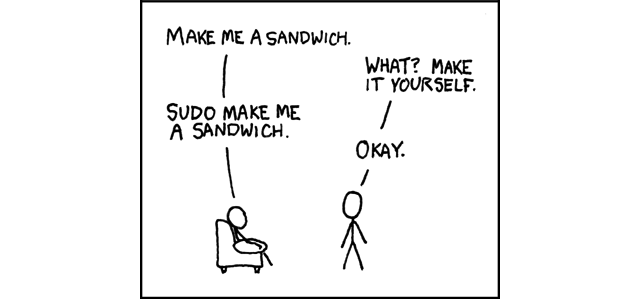
\includegraphics[width=0.6\textwidth]{sandwich.png}
\end{figure}

\section{Environment}\label{sec:env}
\subsection{STDOUT vs STDERR}\label{subsec:STD}
All error messages should go to STDERR.

This makes it easier to separate normal status from actual issues.

A function to print out error messages along with other status information is recommended.

\code{\$*} means all arguments passed into the function or script.

Additionally, you'll notice that the date is set to the ISO 8601 standard.

\inputminted[frame=single,firstline=5, lastline=12,linenos]{bash}{./styleguide.bash}

\section{Comments}
\label{sec:comms}
\subsection{File Header}
\label{subsec:file_header}
Start each file with a description of its contents.

Every file must have a top-level comment including a brief overview of its contents. A copyright notice and author information are optional.

Example:
\inputminted[frame=single,firstline=1, lastline=3,linenos]{bash}{./styleguide.bash}

\subsection{Function Comments}
\label{subsec:func_comms}
Any function that is not both obvious and short must be commented. Any function in a library must be commented regardless of length or complexity.

It should be possible for someone else to learn how to use your program or to use a function in your library by reading the comments (and self-help, if provided) without reading the code.

All function comments should describe the intended API behaviour using:
\begin{itemize}
    \item Description of the function.
    \item Globals: List of global variables used and modified.
    \item Arguments: Arguments taken.
    \item Outputs: Output to STDOUT or STDERR.
    \item Returns: Returned values other than the default exit status of the last command run.
\end{itemize}

Example:

\inputminted[frame=single,firstline=14, lastline=48,linenos]{bash}{./styleguide.bash}

\subsection{Implementation Comments}
\label{subsec:Imp_comms}
Comment tricky, non-obvious, interesting or important parts of your code.

This follows general coding comment practice. Don’t comment everything. If there’s a complex algorithm or you’re doing something out of the ordinary, put a short comment in.

\subsection{TODO Comments}
\label{subsec:todo_comms}
\inputminted[frame=single,firstline=50, lastline=50,linenos]{bash}{./styleguide.bash}

\section{Formatting}
\label{sec:Form}
While you should follow the style that’s already there for files that you’re modifying, the following are required for any new code.

\subsection{Indentation}
\label{subsec:Indent}
Indent 2 spaces. No tabs.

Use blank lines between blocks to improve readability. Indentation is two spaces. Whatever you do, don’t use tabs. For existing files, stay faithful to the existing indentation.

\section{Line Length and Long Strings}
\label{subsec:Line_Len}
Maximum line length is 80 characters.

If you have to write strings that are longer than 80 characters, this should be done with a here document or an embedded newline if possible. Literal strings that have to be longer than 80 chars and can’t sensibly be split are ok, but it’s strongly preferred to find a way to make it shorter.
\inputminted[frame=single,firstline=52, lastline=60,linenos]{bash}{./styleguide.bash}

\subsection{Pipelines}
\label{subsec:pipelines}
Pipelines should be split one per line if they don’t all fit on one line.

If a pipeline all fits on one line, it should be on one line.

If not, it should be split at one pipe segment per line with the pipe on the newline and a 2 space indent for the next section of the pipe. This applies to a chain of commands combined using \code{|} as well as to logical compounds using \code{||} and \code{\&\&}.

\inputminted[frame=single,firstline=62, lastline=69,linenos]{bash}{./styleguide.bash}

\subsection{Loops}
\label{subsec:loops}
Put \code{;} do and \code{;} then on the same line as the \code{while}, \code{for} or \code{if}.

Loops in shell are a bit different, but we follow the same principles as with braces when declaring functions. That is: \code{;} then and \code{;} do should be on the same line as the \code{if}/\code{for}/\code{while}. \code{else} should be on its own line and closing statements should be on their own line vertically aligned with the opening statement.

\inputminted[frame=single,firstline=70, lastline=87,linenos]{bash}{./styleguide.bash}

\subsection{Case Statement}
\label{subsec:case_state}
\begin{itemize}
    \item Indent alternatives by 2 spaces.
    \item A one-line alternative needs a space after the close parenthesis of the pattern and before the \code{;;}.
    \item Long or multi-command alternatives should be split over multiple lines with the pattern, actions, and \code{;;} on separate lines.
\end{itemize}


The matching expressions are indented one level from the \code{case} and \code{esac}. Multiline actions are indented another level. In general, there is no need to quote match expressions. Pattern expressions should not be preceded by an open parenthesis. Avoid the \code{;\&} and \code{;;\&} notations.

\inputminted[frame=single,firstline=89, lastline=101,linenos]{bash}{./styleguide.bash}

Simple commands may be put on the same line as the pattern and ;; as long as the expression remains readable. This is often appropriate for single-letter option processing. When the actions don’t fit on a single line, put the pattern on a line on its own, then the actions, then \code{;;} also on a line of its own. When on the same line as the actions, use a space after the close parenthesis of the pattern and another before the \code{;;}.

\inputminted[frame=single,firstline=103, lastline=115,linenos]{bash}{./styleguide.bash}

\subsection{Variable Expansion}
\label{subsec:var_exp}
In order of precedence: Stay consistent with what you find; quote your variables; prefer \code{"\${var}"} over \code{"\$var"}.

These are strongly recommended guidelines but not mandatory regulation. Nonetheless, the fact that it’s a recommendation and not mandatory doesn’t mean it should be taken lightly or downplayed.

They are listed in order of precedence.
\begin{itemize}
    \item Stay consistent with what you find for existing code.
    \item Quote variables, see \nameref{subsec:quot} section below.
    \item Don’t brace-delimit single character shell specials / positional parameters, unless strictly necessary or avoiding deep confusio
\end{itemize}

Prefer brace-delimiting all other variables.
\inputminted[frame=single,firstline=117, lastline=135,linenos]{bash}{./styleguide.bash}
\begin{center}
\vspace{4em}
\ldots continues overleaf    
\end{center}

\newpage
\inputminted[frame=single,firstline=137, lastline=146,linenos]{bash}{./styleguide.bash}
NOTE: Using braces in \code{\${var}} is not a form of quoting. \code{“Double quotes”} must be used as well.

\subsection{Quoting}
\label{subsec:quot}
\begin{itemize}
    \item Always quote strings containing variables, command substitutions, spaces or shell meta characters, unless careful unquoted expansion is required or it’s a shell-internal integer (see next point).
    \item Use arrays for safe quoting of lists of elements, especially command-line flags. See Arrays below.
    \item Optionally quote shell-internal, readonly special variables that are defined to be integers: \code{\$?}, \code{\$\#}, \code{\$\$}, \code{\$!} (man bash). Prefer quoting of “named” internal integer variables, e.g. PPID etc for consistency.
    \item Prefer quoting strings that are “words” (as opposed to command options or path names).
    \item Never quote literal integers.
    \item Be aware of the quoting rules for pattern matches in \code{[[ … ]]}. See the Test, \code{[ … ]}, and \code{[[ … ]]} section below.
    \item Use \code{"\$\@"} unless you have a specific reason to use \code{\$*}, such as simply appending the arguments to a string in a message or log.
\end{itemize}
\inputminted[frame=single,firstline=148, lastline=169,linenos]{bash}{./styleguide.bash}

\begin{center}
\vspace{1em}
\ldots continues overleaf    
\end{center}
\newpage
\inputminted[frame=single,firstline=171, lastline=212,linenos]{bash}{./styleguide.bash}

\section{Features and Bugs}
\label{sec:feat_bugs}

\subsection{Shell Check}
\label{subsec:shell_check}
The (\url{https://www.shellcheck.net}) project identifies common bugs and warnings for your shell scripts. It is recommended for all scripts, large or small.

\subsection{Command Substitution}
\label{subsec:cmd_sub}
Use \code{\$(command)} instead of backticks.

Nested backticks require escaping the inner ones with \\ . The \code{\$(command)} format doesn’t change when nested and is easier to read.

Example:
\inputminted[frame=single,firstline=214, lastline=218,linenos]{bash}{./styleguide.bash}

\subsection{Test, \code{[[ … ]}, and \code{[[ … ]]}}
\label{subsec:test}
\code{[[ … ]]} is preferred over \code{[ … ]}, test and \code{/usr/bin/[}.

\code{[[ … ]]} reduces errors as no path name expansion or word splitting takes place between \code{[[} and \code{]]}. In addition, \code{[[} … \code{]]} allows for regular expression matching, while \code{[ … ]} does not.

\inputminted[frame=single,firstline=220, lastline=230,linenos]{bash}{./styleguide.bash}

\inputminted[frame=single,firstline=232, lastline=236,linenos]{bash}{./styleguide.bash}

For the gory details, see E14 at \url{http://tiswww.case.edu/php/chet/bash/FAQ} .

\subsection{Testing Strings}
\label{subsec:test_str}
Use quotes rather than filler characters where possible.

Bash is smart enough to deal with an empty string in a test. So, given that the code is much easier to read, use tests for empty/non-empty strings or empty strings rather than filler characters.

\inputminted[frame=single,firstline=238, lastline=252,linenos]{bash}{./styleguide.bash}

\begin{center}
\vspace{1em}
\ldots continues overleaf    
\end{center}

\inputminted[frame=single,firstline=254, lastline=257,linenos]{bash}{./styleguide.bash}

To avoid confusion about what you’re testing for, explicitly use \code{-z} or \code{-n}.

\inputminted[frame=single,firstline=259, lastline=262,linenos]{bash}{./styleguide.bash}

\inputminted[frame=single,firstline=264, lastline=267,linenos]{bash}{./styleguide.bash}

For clarity, use \code{==} for equality rather than = even though both work. The former encourages the use of \code{[[} and the latter can be confused with an assignment. However, be careful when using \code{<} and \code{>} in \code{[[ … ]]} which performs a lexicographical comparison. Use \code{(( … ))} or \code{-lt} and \code{-gt} for numerical comparison.

\inputminted[frame=single,firstline=269, lastline=280,linenos]{bash}{./styleguide.bash}

\inputminted[frame=single,firstline=282, lastline=291,linenos]{bash}{./styleguide.bash}

\subsection{Wildcard Expansion of Filenames}
\label{subsec:wild_file}
Use an explicit path when doing wildcard expansion of filenames.

As filenames can begin with a \code{-}, it’s a lot safer to expand wildcards with \code{./*} instead of \code{*}

\inputminted[frame=single,firstline=293, lastline=299,linenos]{bash}{./styleguide.bash}

\inputminted[frame=single,firstline=301, lastline=306,linenos]{bash}{./styleguide.bash}

\subsection{Eval}
\label{subsec:eval}
\code{eval} should be avoided.

\code{eval} munges the input when used for assignment to variables and can set variables without making it possible to check what those variables were.

\inputminted[frame=single,firstline=313, lastline=308,linenos]{bash}{./styleguide.bash}

\subsection{Arrays}
\label{subsec:arrays}
Bash arrays should be used to store lists of elements, to avoid quoting complications. This particularly applies to argument lists. Arrays should not be used to facilitate more complex data structures (see \nameref{subsec:when_shell} above).

Arrays store an ordered collection of strings, and can be safely expanded into individual elements for a command or loop.

Using a single string for multiple command arguments should be avoided, as it inevitably leads to authors using eval or trying to nest quotes inside the string, which does not give reliable or readable results and leads to needless complexity.

\inputminted[frame=single,firstline=315, lastline=320,linenos]{bash}{./styleguide.bash}

\inputminted[frame=single,firstline=322, lastline=325,linenos]{bash}{./styleguide.bash}

\inputminted[frame=single,firstline=327, lastline=340,linenos]{bash}{./styleguide.bash}

\subsubsection{Array Pros}
\begin{itemize}
    \item Using Arrays allows lists of things without confusing quoting semantics. Conversely, not using arrays leads to misguided attempts to nest quoting inside a string.
    \item Arrays make it possible to safely store sequences/lists of arbitrary strings, including strings containing whitespace.
\end{itemize}

\subsubsection{Array Cons}
Using arrays can risk a script’s complexity growing.

\subsubsection{Array Decision}
Arrays should be used to safely create and pass around lists. In particular, when building a set of command arguments, use arrays to avoid confusing quoting issues. Use quoted expansion – \hspace{8em} \code{"\$\{array[\@]\}"} – to access arrays. However, if more advanced data manipulation is required, shell scripting should be avoided altogether; see \nameref{subsec:when_shell} above.

\subsection{Pipes to While}
\label{subsec:pipes_while}
Use process substitution or the \code{readarray} builtin (bash4+) in preference to piping to \code{while}. Pipes create a subshell, so any variables modified within a pipeline do not propagate to the parent shell.

The implicit subshell in a \code{pipe} to while can introduce subtle bugs that are hard to track down.

\inputminted[frame=single,firstline=342, lastline=350,linenos]{bash}{./styleguide.bash}

Using process substitution also creates a subshell. However, it allows redirecting from a subshell to a \code{while} without putting the while (or any other command) in a subshell.

\inputminted[frame=single,firstline=352, lastline=360,linenos]{bash}{./styleguide.bash}

\begin{center}
\vspace{6em}
\ldots continues overleaf    
\end{center}
\newpage
Alternatively, use the \code{readarray} builtin to read the file into an array, then loop over the array’s contents. Notice that (for the same reason as above) you need to use a process substitution with \code{readarray} rather than a pipe, but with the advantage that the input generation for the loop is located before it, rather than after.

\inputminted[frame=single,firstline=362, lastline=369,linenos]{bash}{./styleguide.bash}
\begin{quote}
    \textcolor{gray}{Note: Be cautious using a for-loop to iterate over output, as in for var in \code{\$(...)}, as the output is split by whitespace, not by line. Sometimes you will know this is safe because the output can’t contain any unexpected whitespace, but where this isn’t obvious or doesn’t improve readability (such as a long command inside \code{\$(...))}, a while read loop or \code{readarray} is often safer and clearer.}
\end{quote}

\subsection{Arithmetic}
\label{subsec:arth}
Always use \code{(( … ))} or \code{\$(( … ))} rather than let or \code{\$[ … ]} or expr.

Never use the \code{\$[ … ]} syntax, the \code{expr} command, or the \code{let} built-in.

\code{<} and \code{>} don’t perform numerical comparison inside \code{[[ … ]]} expressions (they perform lexicographical comparisons instead; see \nameref{subsec:test_str}). For preference, don’t use \code{[[ … ]]} at all for numeric comparisons, use (( … )) instead.

It is recommended to avoid using \code{(( … ))} as a standalone statement, and otherwise be wary of its expression evaluating to zero
\begin{itemize}
    \item particularly with set \code{-e} enabled. For example, \code{set -e; i=0; (( i++ ))} will cause the shell to exit.
\end{itemize}

\inputminted[frame=single,firstline=371, lastline=381, linenos]{bash}{./styleguide.bash}

\inputminted[frame=single,firstline=383, lastline=395, linenos]{bash}{./styleguide.bash}

Stylistic considerations aside, the shell’s built-in arithmetic is many times faster than \code{expr}.

When using variables, the \code{\$\{var\}} (and \code{\$var}) forms are not required within \code{\$(( … ))}. The shell knows to look up var for you, and omitting the \code{\$\{…\}} leads to cleaner code. This is slightly contrary to the previous rule about always using braces, so this is a recommendation only.

\inputminted[frame=single,firstline=397, lastline=416, linenos]{bash}{./styleguide.bash}

\section{Naming Conventions}
\label{sec:name_conv}
\subsection{Function Names}
\label{subsec:func_names}
Lower-case, with underscores to separate words. Separate libraries with \code{::}. Parentheses are required after the function name. The keyword function is optional, but must be used consistently throughout a project.

If you’re writing single functions, use lowercase and separate words with underscore. If you’re writing a package, separate package names with \code{::}. Braces must be on the same line as the function name  and no space between the function name and the parenthesis.

\inputminted[frame=single,firstline=418, lastline=426, linenos]{bash}{./styleguide.bash}

The \code{function} keyword is extraneous when \code{()} is present after the function name, but enhances quick identification of functions.

\subsection{Variable Names}
\label{subsec:var_names}
As for function names.

Variables names for loops should be similarly named for any variable you’re looping through.

\begin{center}
\vspace{1em}
\ldots continues overleaf    
\end{center}

\inputminted[frame=single,firstline=428, lastline=430, linenos]{bash}{./styleguide.bash}

\subsection{Constants and Environment Variable Names}
\label{subsec:con_env_names}
All caps, separated with underscores, declared at the top of the file.

Constants and anything exported to the environment should be capitalized.

\inputminted[frame=single,firstline=432, lastline=436, linenos]{bash}{./styleguide.bash}

Some things become constant at their first setting (for example, via \code{getopts}). Thus, it’s OK to set a constant in \code{getopts} or based on a condition, but it should be made \code{readonly} immediately afterwards. For the sake of clarity \code{readonly} or export is recommended instead of the equivalent declare commands.

\inputminted[frame=single,firstline=438, lastline=444, linenos]{bash}{./styleguide.bash}

\subsection{Source Files}
\label{subsec:source_fles}
Lowercase, with underscores to separate words if desired.

This is for consistency with other code styles in used in industry: \code{maketemplate} or \code{make\_template} but not \code{make-template}.

\subsection{Read-only Variables}
\label{subsec:read_var}
Use \code{readonly} or \code{declare -r} to ensure they’re read only.

As globals are widely used in shell, it’s important to catch errors when working with them. When you declare a variable that is meant to be read-only, make this explicit.

\inputminted[frame=single,firstline=446, lastline=451, linenos]{bash}{./styleguide.bash}

\subsection{Use Local Variables}
\label{subsec:loc_vars}
Declare function-specific variables with \code{local}. Declaration and assignment should be on different lines.

Ensure that local variables are only seen inside a function and its children by using \code{local} when declaring them. This avoids polluting the global name space and inadvertently setting variables that may have significance outside the function.

Declaration and assignment must be separate statements when the assignment value is provided by a command substitution; as the \code{local} builtin does not propagate the exit code from the command substitution.

\inputminted[frame=single,firstline=453, lastline=462, linenos]{bash}{./styleguide.bash}

\inputminted[frame=single,firstline=464, lastline=471, linenos]{bash}{./styleguide.bash}

\subsection{Function Locations}
\label{subsec:func_loc}
Put all functions together in the file just below constants. Don’t hide executable code between functions. Doing so makes the code difficult to follow and results in nasty surprises when debugging.

If you’ve got functions, put them all together near the top of the file. Only includes, set statements and setting constants may be done before declaring functions.

\subsection{main}
\label{subsec:main}
A function called \code{main} is required for scripts long enough to contain at least one other function.

In order to easily find the start of the program, put the \code{main} program in a function called main as the bottom most function. This provides consistency with the rest of the code base as well as allowing you to define more variables as \code{local} (which can’t be done if the main code is not a function). The last non-comment line in the file should be a call to \code{main}:

\inputminted[frame=single,firstline=473, lastline=473, linenos]{bash}{./styleguide.bash}

Obviously, for short scripts where it’s just a linear flow, \code{main} is overkill and so is not required.

\section{Calling Commands}
\label{sec:call_cmds}
\subsection{Checking Return Values}
\label{subsec:check_rt_vals}
Always check return values and give informative return values.

For unpiped commands, use \code{\$?} or check directly via an if statement to keep it simple.

Example:

\begin{center}
\vspace{2em}
\ldots continues overleaf    
\end{center}
\newpage
\inputminted[frame=single,firstline=475, lastline=485, linenos]{bash}{./styleguide.bash}

Bash also has the \code{PIPESTATUS} variable that allows checking of the return code from all parts of a pipe. If it’s only necessary to check success or failure of the whole pipe, then the following is acceptable:

\inputminted[frame=single,firstline=487, lastline=490, linenos]{bash}{./styleguide.bash}

However, as \code{PIPESTATUS} will be overwritten as soon as you do any other command, if you need to act differently on errors based on where it happened in the pipe, you’ll need to assign \code{PIPESTATUS} to another variable immediately after running the command (don’t forget that \code{[} is a command and will wipe out \code{PIPESTATUS}).

\inputminted[frame=single,firstline=492, lastline=499, linenos]{bash}{./styleguide.bash}

\subsection{Builtin Commands vs. External Commands}
\label{subsec:Built_cmds}
Given the choice between invoking a shell builtin and invoking a separate process, choose the builtin.

We prefer the use of builtins such as the \emph{Parameter Expansion} functions in \code{bash(1)} as it’s more robust and portable (especially when compared to things like \code{sed}).

Examples:

\inputminted[frame=single,firstline=501, lastline=503, linenos]{bash}{./styleguide.bash}

\inputminted[frame=single,firstline=505, lastline=507, linenos]{bash}{./styleguide.bash}

\end{document}
